\documentclass[
  11pt,
  letterpaper,
   addpoints,
   answers
  ]{exam}

\usepackage{../exercise-preamble}

\begin{document}

\noindent
\begin{minipage}{0.47\textwidth}

\includegraphics[width=\textwidth]{../fcfm_die}
\end{minipage}
\begin{minipage}{0.53\textwidth}
\begin{center} 
\large\textbf{Fundamentos de control de sistemas} (EL4111-1) \\
\large\textbf{Pauta auxiliar 12} \\
\small Prof.~Roberto Cardenas Dobson\\
\small Prof.~Aux.~Osvaldo Jimenez - Erik Sáez\\
\small Ayudantes.~Simon Arenas- Juan Pablo Baez - Francisco Garces - Sofia Ibarra\\
\end{center}
\end{minipage}

\vspace{0.5cm}
\noindent
\vspace{.85cm}
\begin{questions}
%----------------------------------------------
    \question Se trabaja con el circuito de la Figura 1, donde $L = 15\,\text{mH}$, $C = 2000\,\mu\text{F}$, $R_2 = 200\,\Omega$ y $R_1 = R_3 = 400\,\Omega$. La salida del sistema es la caída de tensión en la resistencia $R_3$. Este circuito es parte de un sistema de comunicaciones que actúa como un filtro pasabanda para separar señales en un canal de transmisión. Sin embargo, el sistema debe ajustarse dinámicamente para cumplir con los requisitos de estabilidad y tiempo de respuesta necesarios para evitar interferencias y mejorar la calidad de la señal. Para ello, se plantea modificar los polos del sistema mediante control.

    \begin{figure}[h!]
        \centering
        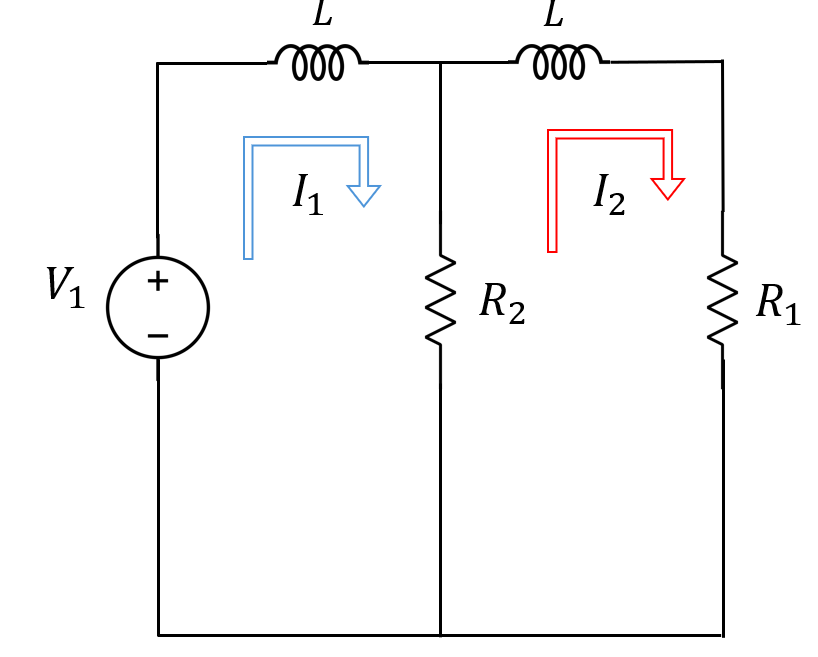
\includegraphics[width=0.75\textwidth]{Examen_1}
        \caption{Circuito eléctrico}
    \end{figure}
    
    \begin{enumerate}
        \item[(a)] Encuentre las ecuaciones de estado del sistema físico, identificando las matrices $\mathbf{A}$, $\mathbf{B}$, $\mathbf{C}$ y $\mathbf{D}$.
        \item[(b)] Determine si el sistema es observable y/o controlable.
        \item[(c)] Utilice la fórmula canónica de control para encontrar una ganancia que permita ubicar los polos del sistema a lazo cerrado en $s^* = -40 \pm j40$. Justifique por qué esta ubicación es adecuada para mejorar las características dinámicas del filtro dentro del sistema de comunicaciones.
        \item[(d)] Reformule sus matrices ahora considerando control integral para la variable que estime conveniente. Justifique en que modifica esto al sistema.
        \item[(e)] En esta ultima situacion que puede decir con respecto a la controlabilidad y observabilidad del sistema.
    \end{enumerate}
%----------------------------------------------
\begin{solution}
    \subsection*{Resolucion 1.1}
    Se busca obtener las ecuaciones de estado del sistema fisico, en base a las mallas propeustas se tiene para la malla 2:
    \begin{align}
        R_{1}(i_{1} + i_{2}) + v_{c} + R_{2}i_{1} + V_{1}=0\\
    \end{align}
    Se tiene ademas que:
    \begin{align}
        (i_{1} + i_{2}) = C \frac{\partial v_{c}}{\partial t}
    \end{align}
    Por lo tanto tenemos que:
    \begin{align}
        R_{1} C \frac{\partial v_{c}}{\partial t} + v_{c} + R_{2}\left( C \frac{\partial v_{c}}{\partial t} - i_{2}\right) + V_{1}&=0\\
        \frac{\partial v_{c}}{\partial t} = \frac{-v_{c}}{C(R_{1}+R_{2})} + \frac{R_{2}}{C(R_{1}+ R_{2})}i_{2} - \frac{V_{1}}{C(R_{1}+R_{2})}
    \end{align} 
    Para la otra malla se tiene: 
    \begin{align}
        R_{1}(i_{1} + i_{2}) + v_{c} + v_{L} + R_{3}i_{2} = 0
    \end{align}
    Donde se tiene que:
    \begin{align}
        v_{L} = L \frac{\partial i_{2}}{\partial t} 
    \end{align}
    Reemplazando $\frac{\partial v_{c}}{\partial t}$ tenemos que:
    \begin{align}
        R_{1} C \left( \frac{-v_{c}}{C(R_{1}+R_{2})} + \frac{R_{2}}{C(R_{1}+ R_{2})}i_{2} - \frac{V_{1}}{C(R_{1}+R_{2})}\right)+ v_{c} + L \frac{\partial i_{2}}{\partial t} + R_{3}i_{2} = 0
    \end{align} 
    Reordenando la expresion se tiene que:
    \begin{align}
        \frac{\partial i_{2}}{\partial t} = -v_{c} \frac{R_{2}}{L(R_{1}+ R_{2})} - i_{2}\left(\frac{R_{3}(R_{1}+R_{2}) + R_{1}R_{2}}{L(R_{1}+R_{2})}\right) + \frac{V_{1}R_{1}}{L(R_{1}+R_{2})} 
    \end{align}
    De esta manera es posible el formular la matriz como:
    \begin{align}
        \begin{bmatrix}
        \frac{\partial v_{c}}{\partial t} \\
        \frac{\partial i_{2}}{\partial t}
        \end{bmatrix} =
        \begin{bmatrix}
        \frac{-1}{C(R_{1}+R_{2})} & \frac{R_{2}}{C(R_{1}+R_{2})} \\
        \frac{-R_{2}}{L(R_{1}+R_{2})} &  
        -\left(\frac{R_{3}(R_{1}+R_{2}) + R_{1}R_{2}}{L(R_{1}+R_{2})} \right)
        \end{bmatrix}
        \begin{bmatrix}
        v_{c} \\
        i_{2}
        \end{bmatrix}
        + V_1
        \begin{bmatrix}
        \frac{-1}{C(R_{1}+R_{2})} \\
        \frac{R_{1}}{L(R_{1}+R_{2})}
        \end{bmatrix}.
    \end{align}        
    Dado que la salida del sistema es la caida de tension en la resistencia $R_{3}$, se tiene que:
    \begin{align}
        V_{R_{3}} = R_{3}i_{2}
    \end{align}
    En forma matricial se tiene que:
    \begin{align}
        V_{R_{3}} = \begin{bmatrix}
            0 & R_{3}
        \end{bmatrix} \begin{bmatrix}
            v_{c} \\
            i_{2}
        \end{bmatrix}
    \end{align}
    De esta manera se identifican todas las matrices del sistema.
    \subsection{Resolucion 1.2}
    Por tanto se tiene que:
    \begin{align}
        A &=
        \begin{bmatrix}
        -0.833 & 166.67 \\
        -22.22 & -35555.56
        \end{bmatrix}, \\
        B &=
        \begin{bmatrix}
        -0.833 \\
        44.444
        \end{bmatrix}, \\
        C &=
        \begin{bmatrix}
        0 & 400
        \end{bmatrix}.
    \end{align}
    Luego se busca analizar tanto controlabilidad como observabilidad del sistema, para ello se calcula la matriz de controlabilidad:
    \begin{align}
        \mathcal{C} = \begin{bmatrix}
            B & AB
        \end{bmatrix} = \begin{bmatrix}
            -0.833 & 7408.18 \\
            44.444 & -1580212.80
        \end{bmatrix}
    \end{align}    
    Luego su determinante sera:
    \begin{align}
        det(\mathcal{C}) = 987068.32
    \end{align}
    Por lo tanto el sistema es controlable. Luego se calcula la matriz de observabilidad:
    \begin{align}
        \mathcal{O} = \begin{bmatrix}
            C \\
            CA
        \end{bmatrix} = \begin{bmatrix}
            0 & 400 \\
            -8888 & -14222224
        \end{bmatrix}
    \end{align}
    Su determinante sera:
    \begin{align}
        det(\mathcal{O}) = 3555552
    \end{align}
    Por lo tanto el sistema es observable.
    \subsection{Resolucion 1.3}
    Se busca ubicar los polos del sistema en $s^{*} = -40 \pm j40$, para ello se busca la matriz de ganancia $K$ que permita ubicar los polos en la ubicacion deseada. Para ello se tiene que:
    \begin{align}
        det(sI - (A - BK)) = 0
    \end{align}
    Por lo tanto se tiene que para una entrada u= -Kx, se tiene que:
    \begin{align}
        K = \begin{bmatrix}
            k_{1} & k_{2}
        \end{bmatrix}
    \end{align}
    De esta manera se obtiene que:
    \begin{align}
        \det(sI - (A - BK)) = \lambda^2 &+ (35556.393 - 0.833k_1 + 44.444k_2)\lambda \\
        &+ (33321.18888 - 22210.3k_1 + 55.531112k_2).
    \end{align}
    Luego tenemos que los polos buscados son $s^{*} = -40 \pm j40$, por lo tanto se tiene que:
    \begin{align}
        (\lambda + 40 - j40)(\lambda + 40 + j40) = \lambda^2 + 80\lambda + 3200
    \end{align}
    Con esto se forma un sistema de ecuaciones:
    \begin{align}
        35556.393 - 0.833k_1 + 44.444k_2 &= 80\\ 
        33321.18888 - 22210.3k_1 + 55.531112k_2 &= 3200
    \end{align}
    De esta manera tenemos los valores que:
    \begin{align}
        k_1 &= -0.640, \\
        k_2 &= -798.239.
    \end{align}
    Con lo que se obtiene el control, tambien se puede realizar mediante la matriz de controlabilida (Es valido)
    \subsection{Resolucion 1.4}
    Se busca ahora reformular las matrices del sistema considerando control integral para la variable $v_{c}$, por lo que se tiene que:
    \begin{align}
        \begin{bmatrix}
        \frac{\partial v_{c}}{\partial t} \\
        \frac{\partial i_{2}}{\partial t} \\
        \frac{\partial v_{c_{i}}}{\partial t}
        \end{bmatrix} &=
        \begin{bmatrix}
        -0.833 & 166.67 & 0 \\
        -22.22 & -35555.56 & 0 \\
        1 & 0 & 0
        \end{bmatrix}
        \begin{bmatrix}
        v_{c} \\
        i_{2} \\
        v_{c_{i}}
        \end{bmatrix} \\
        &\quad + V_1
        \begin{bmatrix}
        -0.833 \\
        44.444 \\
        0
        \end{bmatrix}
        + 
        \begin{bmatrix}
        0 \\
        0 \\
        -1
        \end{bmatrix} v_{c_{1}}^{*}.
    \end{align}
    \subsection{Resolucion 1.5}
    Con respecto a la controlabilidad y observabilidad del sistema, se puede hablar de que el sistema es controlable y observable, y ademas tenemos un control integral. En el caso hipotetico en que no se pudiera observar alguna variable es posible el realizar un observador y que permite realizar un controlador con la variable no observable.
\end{solution}
%----------------------------------------------

\end{questions}
\newpage
%%%%%%%%%%%%%%%%%%%%%%%%%%%

\end{document}